\chapter{Diagramme de séquence}

\section{Diagramme}

\begin{figure}
  \centering
  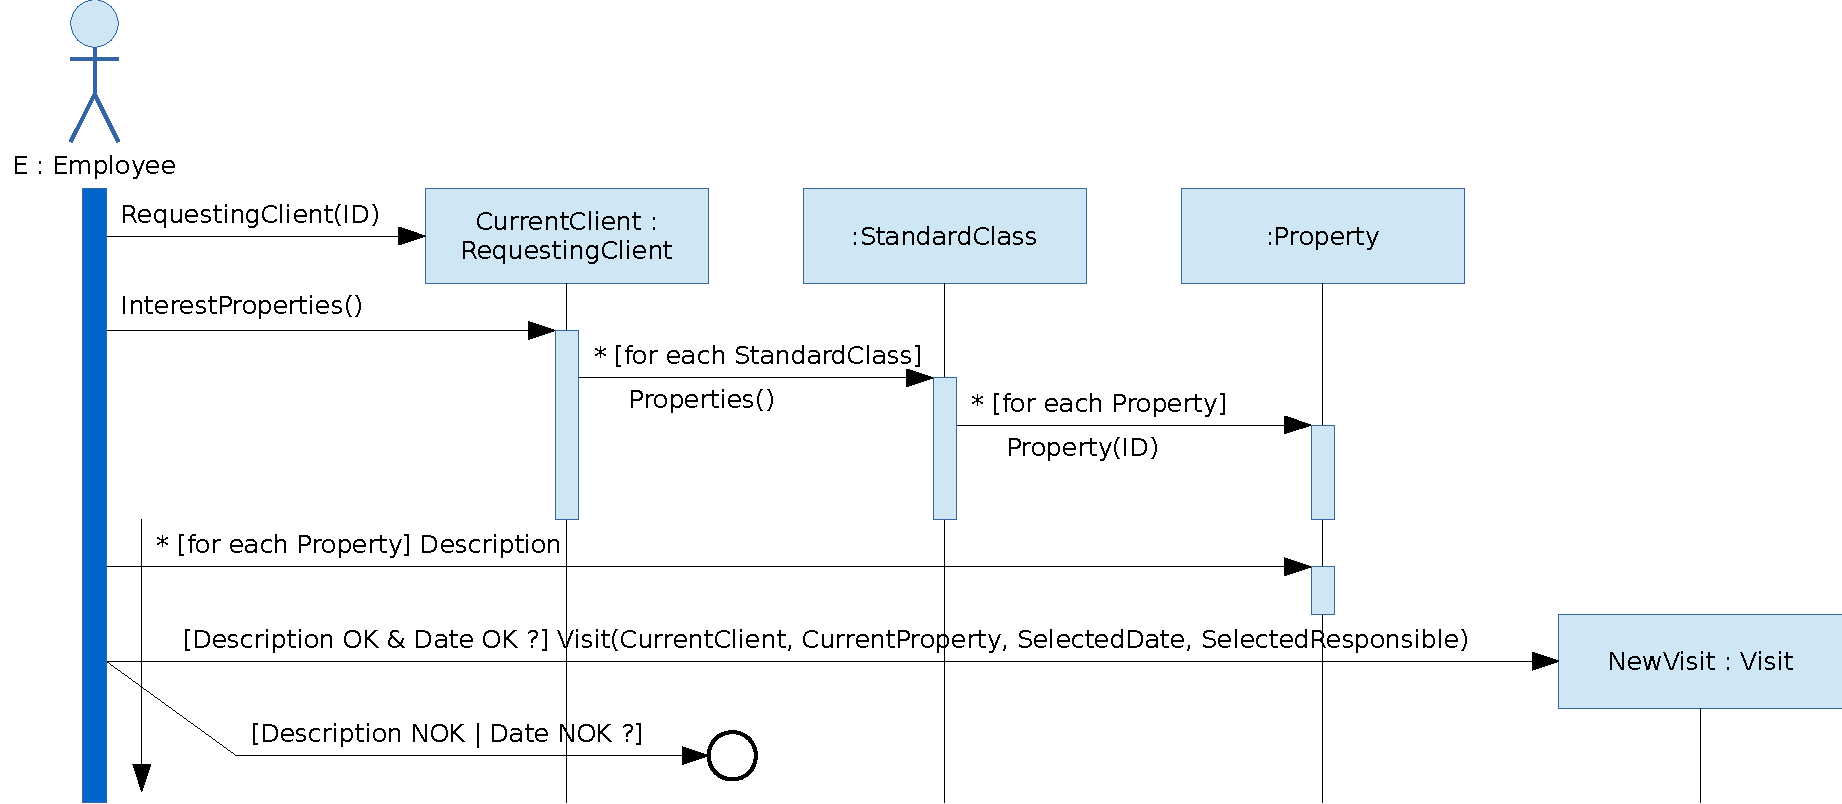
\includegraphics[scale=0.67,angle=90]{IMG/id}
  \caption{Diagramme de séquence}
  \label{img_id}
\end{figure}

La figure \refpage{img_id} illustre le diagramme de séquence du cas d'utilisation \selectedusecase{}.

\section{Rapport}

Ce diagramme est basé sur le diagramme d'activité du cas d'utilisation \selectedusecase{} et le diagramme de classes. Ce diagramme permettra d'avoir une vision sur la manière dont les classes interagissent entre elles pour ce cas d'utilisation ainsi que la manière dont il sera implémenté.